\documentclass[hyperref={pdfpagelabels=false}]{beamer} %weil ist blöde und kann pdfpagelabels im beamer nicht aber versucht es trotzdem
\usepackage[utf8x]{inputenc} %soll utf8 als code verwenden
\PrerenderUnicode{äöüÄÖÜß} % umlaute gehen nun auch

\usepackage[ngerman]{babel} % deutsche Bezeichnungen

\usepackage{amsmath} % mathe formeln
\usepackage{amsthm} % mathe theoreme
\usepackage{graphicx} % Darstellung von Bildern

% - Times, Helvetica, Courier (Word Standard...)
\usepackage{mathptmx}
\usepackage[scaled=.90]{helvet}
\usepackage{courier}

\usepackage{beamerthemesplit} % das theme

% neue Theorem Blöcke
\newtheorem{thm}{Theorem}
\newtheorem{defin}{Definition}
\newtheorem{lem}{Lemma}
\newtheorem{beh}{Behauptung}

\title{Monotone vs. Non-monotone Circuit Complexity}
\author{Johannes Honke, Marko Jahn, Stephan Mielke}
\institute{BTU-Cottbus}
\date{20.09.2010}

\begin{document}

  \begin{frame}[plain]
    \titlepage
    \tableofcontents
  \end{frame}

  \section{Einführung: Funktionen}
  \begin{frame} %Stephan
    \frametitle{boolesche Funktionen}
    Eine Funktion ist eine Abbildung von einer Menge A in eine Menge B.\\
    In unserem Fall: $f: \{0,1\}^{n} \rightarrow \{0,1\}$ \\
    Also jedes Tupel von Elementen der Menge A $\{0, 1\}$ wird genau auf ein Element der Menge B $\{0, 1\}$ abgebildet.
  \end{frame}

  \section{monotone Funktionen}
  \subsection*{Definition}
  \begin{frame}%Stephan
    \frametitle{Definition von Monotonie}
    Monotonie ist eine Eigenschaft von Funktionen.\\
    $f:A \rightarrow B: \forall x_1,x_2 \in A : (x_1 \leq_A x_2 \Rightarrow f(x_1) \leq_B f(x_2))$\\
    Um die Mengen ordnen zu können, brauchen wir Ordnungsrelationen.\\
    Wir benutzen hier das Symbol $\leq_A$ für die Ordnungsrelation über die Menge $A$ und $\leq_B$ für die der Menge $B$.
  \end{frame}

  \subsection*{Allgemeine Beispiele}
  \begin{frame}
    \frametitle{Beispiele}
    Allgemeine Beispiele für monotone Funktionen:\\
    \begin{tabular}[t]{ll}
      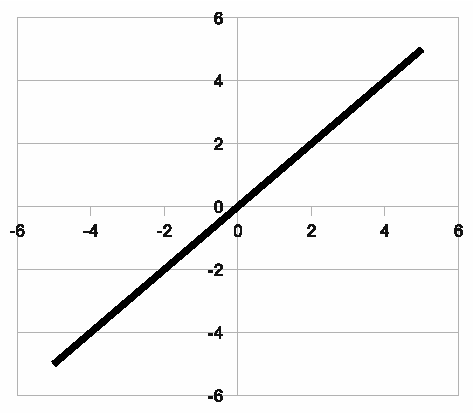
\includegraphics[scale=0.35]{images/f1.pdf} & $f(x) = m * x + n$
    \end{tabular}
    \\Beispiele für NICHT monotone Funktionen:\\
    \begin{tabular}[t]{ll}
      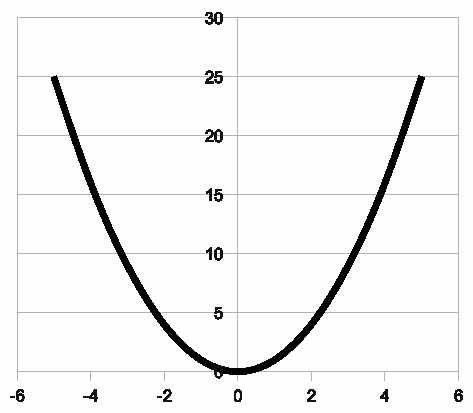
\includegraphics[scale=0.35]{images/f2.pdf} & $f(x) = a * x^2 + b * x + c$
    \end{tabular}
  \end{frame}

  \subsection{Ordnungsfunktionen}
  \begin{frame}%Stephan
    \frametitle{Ordnungsfunktionen}
    Die monotone Eigenschaft von Funktionen wird durch 3 partielle Ordnungen erfüllt.
    \begin{itemize}
      \item reflexiv $\forall a \in A: (a,a) \in B$\\
      \item transitiv $\forall a,b,c \in A: (a,b) \in B \land (b,c) \in B \Rightarrow (a,c) \in B$\\
      \item antisymmetrisch $\forall a,b \in A: (a,b) \in B \land (b,a) \in B \Rightarrow a=b$\\
    \end{itemize}
    Es ergeben sich z.B. folgende monotone Grundfunktionen:\\
    \begin{tabular}[t]{|cc|c|c|c|c|c|c|} \hline
      \multicolumn{2}{|c|}{Menge $A$} & \multicolumn{6}{|c|}{Menge $B$} \\ \hline
      $x_1$     & $x_2$ & AND   & OR    & 0     & 1     & $p_1$ & $p_2$\\ \hline
      0         & 0     & 0     & 0     & 0     & 1     & 0     & 0\\
      0         & 1     & 0     & 1     & 0     & 1     & 0     & 1\\
      1         & 0     & 0     & 1     & 0     & 1     & 1     & 0\\
      1         & 1     & 1     & 1     & 0     & 1     & 1     & 1\\ \hline
    \end{tabular}
  \end{frame}

  \subsection{Ordnungsrelations-Beispiele}
  \subsubsection*{Ordnungsrelation Beispiel der Tupel mit n = 1}
  \begin{frame}
    \begin{figure}
      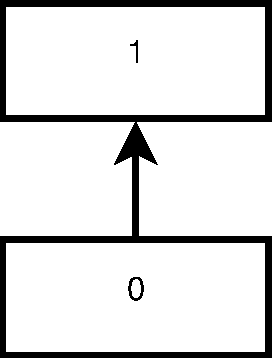
\includegraphics[scale=0.30]{images/m1.pdf}
      \caption{Anstieg der Tupel mit n = 1}
      Die Ordnungsrelation ist einfach von Unten nach Oben ablesbar.
    \end{figure}
  \end{frame}

  \subsubsection*{Ordnungsrelation Beispiel der Tupel mit n = 2}
  \begin{frame}
    \begin{figure}
      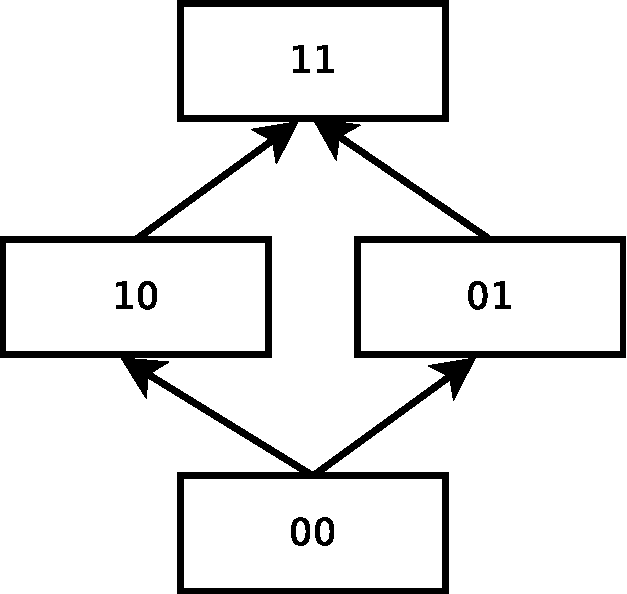
\includegraphics[scale=0.30]{images/m2.pdf}
      \caption{Anstieg der Tupel mit n = 2}
      Die Ordnungsrelation ist einfach von Unten nach Oben ablesbar.
    \end{figure}
  \end{frame}

  \subsubsection*{Ordnungsrelation Beispiel der Tupel mit n = 3}
  \begin{frame}
    \begin{figure}
      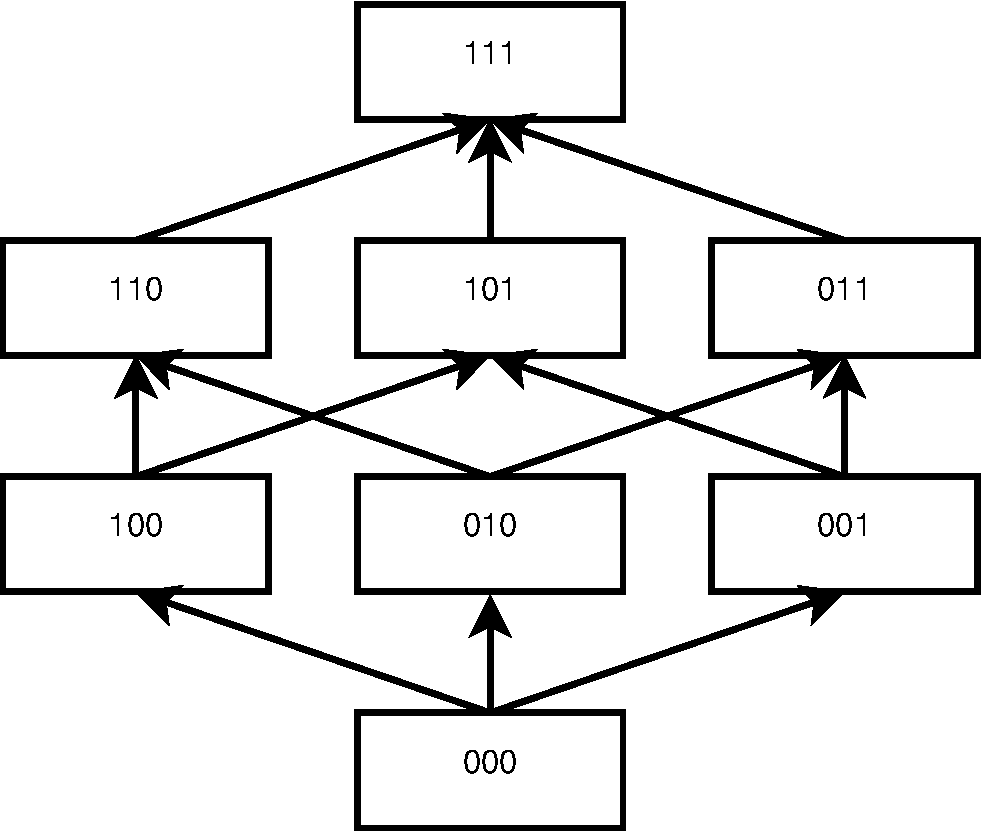
\includegraphics[scale=0.30]{images/m3.pdf}
      \caption{Anstieg der Tupel mit n = 3}
      Die Ordnungsrelation ist NICHT mehr einfach von Unten nach Oben ablesbar, weil das Tupel $010$ und $101$ nicht die 3 partiellen Ordnungen erfüllen.
    \end{figure}
  \end{frame}

  \subsubsection*{Ordnungsrelation Beispiel der Tupel mit n = 4}
  \begin{frame}
    \begin{figure}
      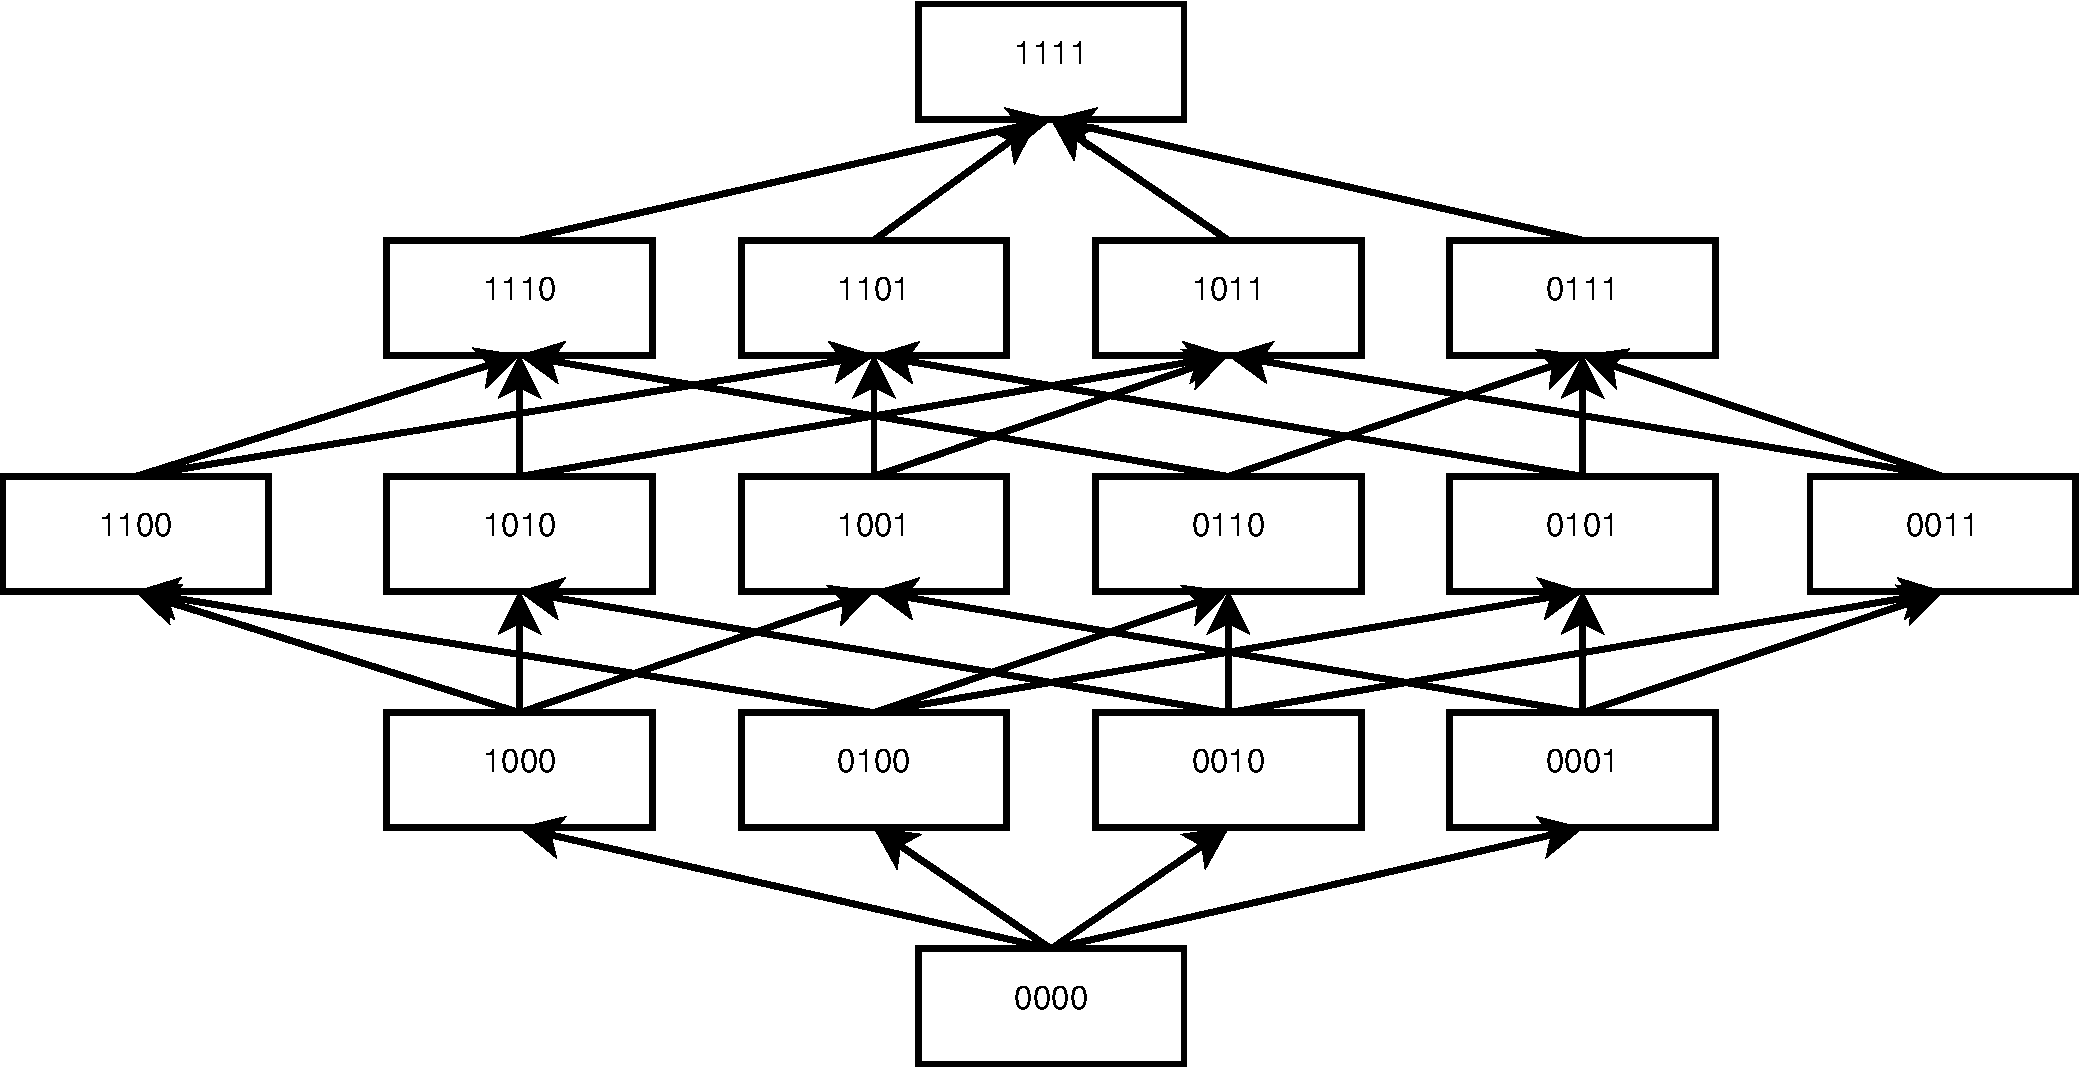
\includegraphics[scale=0.30]{images/m4.pdf}
      \caption{Anstieg des Tupels n = 4}
      Die Ordnungsrelation ist komplexer geworden, da viele Tupel nicht mit denen der höheren Ebene die 3 partiellen Ordnungen erfüllen.
    \end{figure}
  \end{frame}

  \section{Fragen und Antworten}
  \begin{frame}%Marko
    \frametitle{Fragen und Antworten}
    \begin{block}{Gibt es für jede monotone Funktion einen monotonen Schaltkreis?}
      Ja, die DNF besteht zwar aus NOT-Gattern, jedoch, wenn die Funktion monoton war, bleibt die Funktion bestehen, wenn man alle verneinten Variablen entfernt.
    \end{block}
    \begin{block}{Berechnet jeder monotone Schaltkreis eine monotone Funktion?}
      Ja, da der Schaltkreis nur aus monotonen Grundgattern (AND, OR, 0, 1 und die Projektionen) bestehen darf, ist die daraus folgende Funktion auch immer monoton.
    \end{block}
  \end{frame}

  \section{Komplexität}
  \subsection*{in Worten}
    \begin{frame}%Johanes
    \frametitle{Komplexität in Worten}
    Die Komplexität ist ein Maß für den Aufwand einer Funktion.
    Dieser Aufwand stellt sich in Grö\ss{}e und Länge der booleschen Funktion dar, die durch einen Schaltkreis auf einem Chip realisiert werden soll.
    Je grö\ss{}er eine Funktion ist, desto mehr Platz brauch sie durch ihre Gatter auf dem Chip und je länger sie ist, desto mehr Zeit braucht ein Signal vom Anfang zum Ende des Schaltkreises.
  \end{frame}

  \subsection*{in Formeln}
  \begin{frame}
    \frametitle{Komplexität in Formeln}
    \begin{itemize}
      \item $G(S)$ berechnet die Anzahl der Gatter des Schaltkreises
      \item $C(f) = min \{G(S) |$ S berechnet f$\}$
      \item $S(f)$ berechnet den kleinstmöglichen Schaltkreis für $f(x)$
      \item $C_M(f) = min \{G(S_M(f))\}$
      \item $S_M(f)$ berechnet den kleinstmöglichen monotonen Schaltkreis
    \end{itemize}
  \end{frame}

  \subsection{Theorem von Tardos}
  \begin{frame}
    \frametitle{Theorem von Tardos}
    Für den Unterschied zwischen einem monotonen und einem nicht monotonen Schaltkreis in Bezug auf die Größe gilt, das seine nicht monotone Variante die untere Schranke für den Monotonen bildet.
    \begin{thm}[Tardos]
      Der Abstand zwischen $C_{M}$ und $C$ ist exponentiell. %glaube ist eine bessere \"Ubersetzung
    \end{thm}
    Der Abstand w\"achst exponentiell mit der Gr\"o\ss{}e des Schaltkreises.
  \end{frame}

  \section{Slice-Funktionen}
  \subsection*{Definition}
  \begin{frame}%Marko
    \frametitle{Definition von Slice-Funktionen}
    \begin{defin}
      Eine Funktion $f:\{0,1\}^n \rightarrow \{0,1\}$ ist eine Slice-Funktion, wenn es ein $k \in \mathbb{N}$ gibt sodass gilt:\\
      $\sum_{i=1}^{n} x_i<k\Rightarrow f(x)=0$\\
      $\sum_{i=1}^{n} x_i>k\Rightarrow f(x)=1$\\
    \end{defin}
    Eine boolesche Funktion ist eine Slice(teilbare)-Funktionen,wenn sie sich monoton verh\"alt.
    Das $k$ gibt an wie viele Eing\"ange auf $1$ stehen m\"ussten damit der Ausgang $1$ wird.
  \end{frame}

  \subsection*{die Monotonie}
  \begin{frame}
    \frametitle{Monotonie von Slice-Funktionen}
    Für eine gegebene Funktion $f:\{0,1\}^n \rightarrow \{0,1\}$ ist der $k-te$ Slice von $f$, $f^{(k)}$ wie folgt definiert:\\
    \begin{defin}
      \begin{align*}
        f^{(k)}(x) =
        \begin{cases}
          0 & \sum\nolimits_{i=1}^{n} x_i < k\\
          1 & \sum\nolimits_{i=1}^{n} x_1 > k\\
          f(x) & \sum\nolimits_{i=1}^{n} x_i = k % gucken ob i=1 oder i_1 gemeint war. weil es ist schon etwas komisch so gewesen.
        \end{cases}
      \end{align*}
    \end{defin}
    Der $k-te$ Slice einer booleschen Funktion ist immer monoton.
  \end{frame}

  \subsection{im Schaltkreis}
  \begin{frame}%Johanes
    \frametitle{Slice-Funktionen im Schaltkreis}
    \begin{lem}
      Für jeden $U_2$ (nicht monotonen) Schaltkreis $\beta$ gibt es einen äquivalenten monotonen Schaltkreis, welcher höchstens
      2 mal so groß ist wie $\beta$. Bei dem f\"ur jeden Eingang auch sein Inverses bereitgestellt wird.
    \end{lem}
  \end{frame}

  \subsection{die Komplexität}
  \begin{frame}%Stephan
    \frametitle{die Komplexität von Slice-Funktionen}
    \begin{beh}
      $C(f) \leq C(f^{(0)}, f^{(1)}, \dots ,f^{(n)})+h(n)$\\
      $f \in U_2; f^{(k)}$ ist der k-te Slice
    \end{beh}
    \begin{itemize}
      \item $C(f^{(0)}, f^{(1)}, \dots ,f^{(n)})$ ist die Gesamtkomplexität für den SK, der alle Slice-Funktionen $f^{(k)}$ von $f(x)$ gleichzeitig berechnet
      \item $h(n) \in \mathbb{N}$ die benötigte Komplexität für den Demultiplexer, der das Ergebnis ausw\"ahlt
      \item $h \in \mathcal{O}(n)$
      \item $n$ Anzahl der Eingänge
    \end{itemize}
  \end{frame}

  \subsection*{Schranken der Komplexität}
  \begin{frame}%Marko
    \frametitle{Grenzen der Komplexität von Slice-Funktionen}
    \begin{thm}
      Wenn $f$ eine Slice-Funktion ist, dann gilt:
      $C(f) \leq C_M(f) \leq (C(f) +n^2 log\;n)$%9.5 Marko
    \end{thm}
    Die untere Schranke von $C_M(f)$ ist $C(f)|f \in U_2$ und die obere $C(f) + n^2 + log n$.
  \end{frame}

  \subsection*{Schwellenwertfunktion}
  \begin{frame}%Marko         ab hier  meine änderungen
     \frametitle{Schwellenwertfunktion}
     Die Schwellenwertfunktion $ T^{n-1}_k(X_i)$\\
     wobei: \\
     $X$ die Menge aller Eingänge des SK ist.\\
     $X_i = X- x_i$
     \begin{defin}
       \begin{align*}
       T^{n-1}_k (X_i)=
       \begin{cases}
         0 & \sum\nolimits_{j=1}^{n} x_j < k\\
         1 & \sum\nolimits_{j=1}^{n} x_j > k\\
         \overline{x_i} & \sum\nolimits_{j=1}^{n} x_j = k
        \end{cases}
       \end{align*}
      \end{defin}
  \end{frame}

  \section{Zusammenfassung}
  \begin{frame}
    \frametitle{behandelte Themen}
    \begin{itemize}
      \item Monotonie
      \item Komplexität
      \item Slice-Funktionen
      \begin{itemize}
        \item im Schaltkreis
        \item Komplexität
        \item Grenzen der Komplexität
      \end{itemize}
    \end{itemize}
  \end{frame}

\end{document}